\chapter{操作系统探索}

\section{操作系统的诞生}

\subsection{第一代:真空管}

操作系统最初出现的场景是一个工程师小组设计、建造一台机器,之后使用机器语言编写程序并通过将上千根电缆接到插线板上连接成电路,
控制机器的基本功能,进而操作机器运算诸如制作正弦、余弦、对数表或计算炮弹弹道的简单数学运算。

这里的人工拔插电缆就充当着操作系统的角色——根据程序直接操作硬件使其运算得出结果。

\subsection{第二代:晶体管}

在晶体管发明后,计算机可靠程度大大增加,计算机开始被一些公司、政府部门或大学使用。

改进后出现了操作系统的载体,卡片和较后期磁带打孔纸带。

由于打孔纸带是分次读入,一次只能读入一个的作业,出现了批处理系统如图~\ref{fig:btss}~\ref{tanenbaum2009modern}: 

\begin{figure}[h]
  \centering
  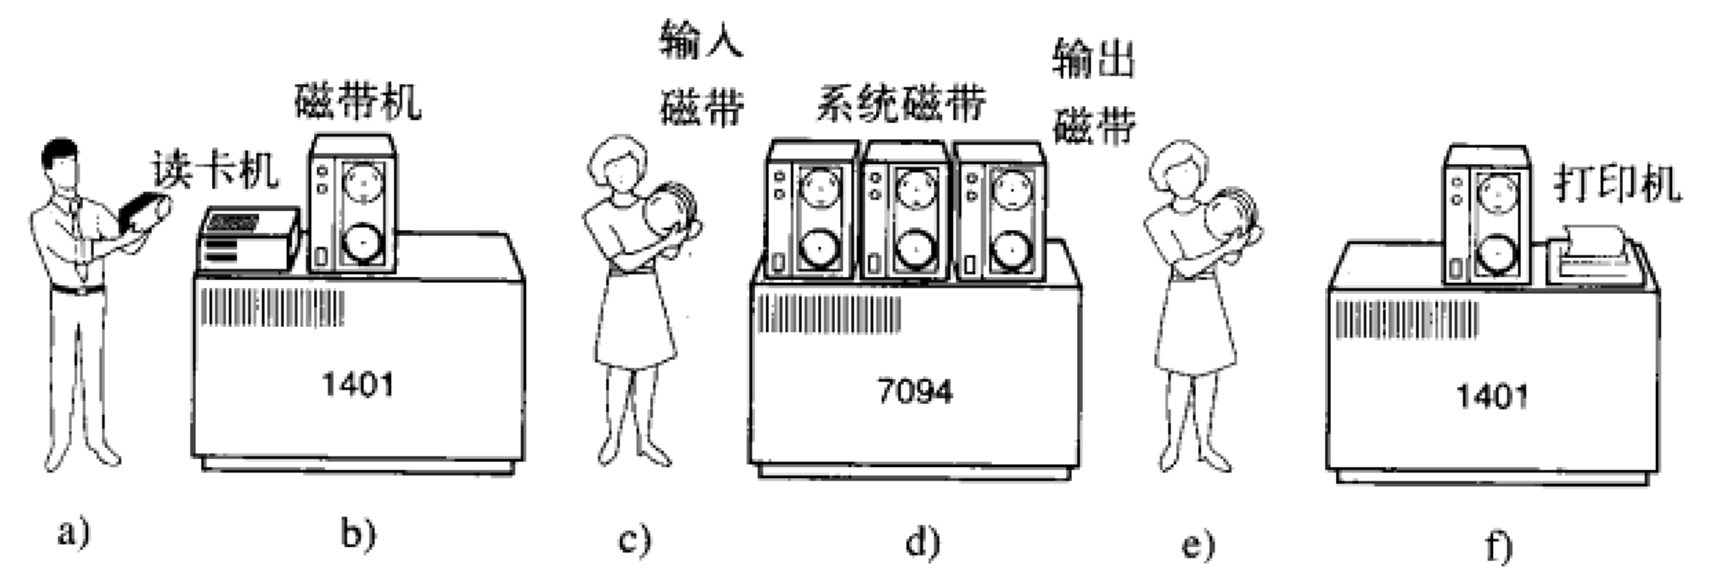
\includegraphics[width=.8\textwidth]{fig/btss.png}
  \caption{批处理系统}
  \label{fig:btss}
\end{figure}

\begin{description}
\item[a.]程序员将打孔纸带拿到1401机\footnote{IBM 1401:数据处理计算机\cite{ibm1401}}
\item[b.]1401机将批处理作业读到磁带上
\item[c.]操作员将输入磁带送至7094机\footnote{IBM 7094:专为大型科学计算而设计,具有出色的性价比和扩展的计算能力\cite{ibm7094}}
\item[d.]7094机进行计算
\item[e.]操作员将输出磁带送到1401机
\item[f.]1401机打印输出
\end{description}

在这里,操作系统的工作已经由完全的人工转换到一部分人工操作交由机器完成,工作效率较之前大大提高,
并且,由于加入了磁带,计算机完成的工作也将及时得到保存。

操作系统的工作已经开始有一定的流程化了。

\subsection{第三代:集成电路}

采用集成电路的第三代计算机较分立晶体管的第二代计算机在性能/价格比上有了很大的提高,

第三代操作系统也加入了多道程序设计和分时系统。

多道程序设计主要目的是解决CPU因等待磁带或其他I/O操作而暂停工作,多道程序设计可以使CPU在程序a的I/O操作时运行程序b。

分时系统解决的主要问题是多用户使用分离的终端,却操作同一台计算机。

\subsection{第四代:个人计算机}

大规模集成电路进一步减小了计算机的大小

\subsection{第五代:移动计算机}

\section{操作系统的规范化}